\section{Datenverarbeitung}
	
	In diesem Kapitel wird näher auf den Programmcode des vorliegenden Forschungsprojektes eingegangen und erklärt was genau wir in der Datensammlung und 
	Datenverarbeitung gemacht wurde. 
	Als erstes haben wir die Daten wie in Punkt 2.1.1 beschrieben mit der Bibliothek gescrapped und als csv-Datei abgespeichert. Wie das Sracpping in der 
	Bibliothek genau funktioniert ist ebenfalls unter dem Punkt 2.1.1. GetOldTweets beschrieben. Um die gespeicherten Tweets für das Mapreduce vor zu 
	verarbeiten nutzen wir die zur Verfügung stehenden Bibliotheken NLTK und cleantext.
	
	
	Die Variable "directory" und "directory_Sanitized" geben den Path an, in welchen Ordner die Daten gespeichert werden sollen. mit der bibliothek os von Python 
	kann man zum Beispiel über "os.listdir(Path)" alle Dateinamen innerhalb dieses Ordners einlesen lassen. 
	Über die Variable user_file_names bekommen wir eine Alphanumerisch sortierte Liste der Usernamen der Politiker zurück, welche wir dann über eine For-
	Schleife durchgehen, da der Name der CSV-Dateien folgenden Muster entspricht, "Name_D" oder "Name_R". D steht für demokratisch und R für 
	republikanisch. In dieser Datensanierungsschleife wird die Funktion tweetDecomposer verwendet. Diese Funktion übernimmt in der vorliegenden Datensanierung die 
	Hauptaufgabe. 
	
	
	- Was genau haben wir alles bei der Datensanierung gemacht?\\
	- Wie haben wir das ganze gemacht? --> Erklären anhand von Ausschnitten unseres Programmcodes\\\\\\
	
	- Was musste berücksichtigt werden?\\
	- Was hat uns Schwierigkeiten bereitet?	
	
	
	\subsection{Sanitization}
	

	
	\begin{figure}[ht]
		\centering
		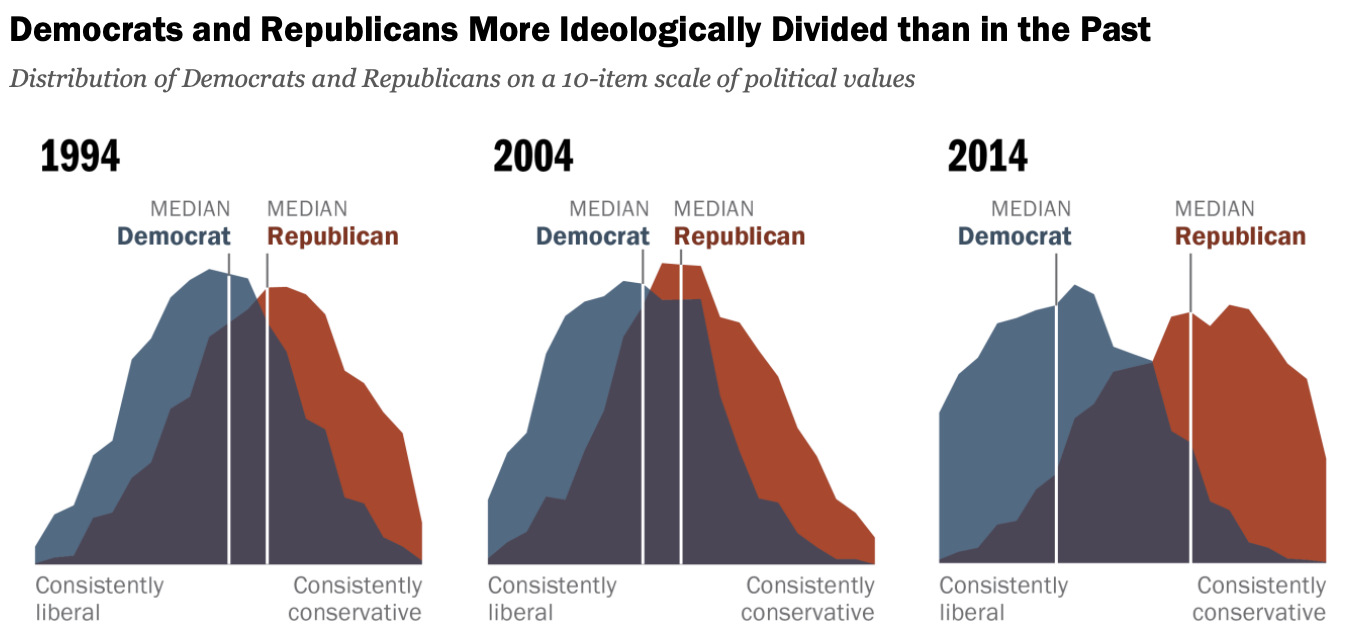
\includegraphics[width=0.9\textwidth]{images/Kapitel1/PoliticalPolarization}
		\captionof{figure}{Ine Beschreibung f}
	\end{figure}
	
	
